To establish the validity of future simulations using current software tools, these tools were benchmarked against background rates measured at HERA, following the luminosity upgrade.  By replicating HERA conditions, simulations produced background rates that were comparable to those recorded in HERA's C5 detector.  Successfully reproducing these rates validates several software tools for background studies and underscores both the need and readiness to conduct JLEIC background studies at this time.

\subsection{HERA Background}
%originally "HERA Issues and Lessons"
Following the HERA-II upgrade in 2000 and 2001, high levels of beam-induced background were observed and identified: synchrotron radiation, proton gas scattering, lepton gas scattering, and proton beam halo losses.   In fact, 95\% of background observed following the upgrade came from proton beam-gas interactions where vacuum conditions had deteriorated due to synchrotron radiation.  The background impacted the detectors and necessitated a several month shutdown to perform simulations and remediate the problem.

%Discuss HERA design elements which made problem worse.
%Several design choices exacerbated the background generated around the IP.  For instance, the electron and proton beams shared the same pipe, which [...].  

%Discuss response, solutions.

During the shutdown, the HERA team performed detailed simulations of the dynamic pressure profile and residual beam gas analysis to determine the best mitigation strategies.  Results indicated that vacuum pressure, dominated by hydrogen gas, spiked to $10^{-8}$ mbar in the region spanning $\pm$ 5 m around the IP.   This  was 100 times higher than the nominal pressure of $10^{-10}$ mbar achieved at the location of the vacuum pumps.  Beam particles interacted with the hydrogen gas, producing halo particles which constituted a large portion of the background events reaching the ZEUS detector.  The C5 counter was placed very close to the beam pipe to measure the rate and arrival times of these halo particles.
%%Insert pictures of vacuum and gas analyses

\subsection{Detector Geometry}

The C5 detector was a silicon tungsten sandwich counter comprised of eight scintillator tiles mounted in pairs above and below the beampipe, orthogonal to the z axis.  The arrangement of the 3 mm thick tiles created an octagon with an outer profile of 20 cm by 20 cm, as shown in Figure \ref{fig:hera5}.  The detector was positioned 1240 mm upstream from the IP around the cylindrical aluminum beampipe of radius 19 mm.  
%insert pictures of C5 Detector placement

\subsection{Detector Rates}
The primary uses of the C5 detector were:
\begin{itemize}
	\item to detect the presence of halo particles in order to reduce background event rates in ZEUS.
	\item to provide rate and arrival time measurements for monitoring and controlling HERA beam conditions.
	\item to calculate the $Z$ vertex position.
\end{itemize}
Figure \ref{fig:hera3} shows the C5 rates as a function of HERA electron beam current for several proton beam currents.  Although the rates in the C5 varied as a function of current, they provide a range by which to base the benchmarking study.  Figure \ref{fig:hera3} indicates that the rate in the C5 detector was approximately 10 kHz for I$_{p}$ = 40 mA, for I$_{e+}$ between 2 mA and 7 mA. 
%insert c5 rates

\subsection{Approach}

In order to benchmark simulation tools against the observed background rates, a virtual detector was modeled after the C5 detector and positioned at the same location relative to the IP.  A beam pipe with the same specifications as the original was filled with a hydrogen target of density proportional to the vacuum quality of the corresponding region at HERA.  

Key parameters were either matched to the HERA case, scaled, or shown to exert little influence over the event rate.  These are summarized below:
% note I = 40 mA matches the C5 rate graph, but nominal energy at the time was 100 mA.  Looks like our calculations are based on 100 mA as well. This might be something to fix as work is finalized.
\begin{center}
	\begin{tabular}{ l l l } 
		   & HERA & Simulated \\ 
		\hline \hline
		Gate Time & 96 ns & 100 ns \\ 
		$p$ bunch length & 100 mm & n/a \\ 
		$I_p$ & 40 mA & 100 mA\\
		$E_p$ (GeV)& 920 & 100, 900 $\pm$ 1 \\
		$N$/bunch & $10^{11}$ & $10^{11}$\\
		$N$ Events & n/a & $\approx 10^6$\\
		vacuum near IP& $10^{-8}$ mbar  & 1 g/cm$^3$ H \\
		Vacuum else& $10^{-10}$ mbar & 0.01 g/cm$^3$ H\\
		Gas & 95\% H & 100\% H\\
		\hline
	\end{tabular}
\end{center}


To replicate the C5 detector, a two-disc scintillator detector was built in GEMC and placed 1240 mm upstream from the IP.  Like the actual C5 detector, the virtual detector was comprised of discs 3 mm thick, separated by 20 mm.  The inner and outer radii also matched the original: $R_{in} = 3.801/2$ cm and $R_{out} = 20.0/2$ cm.  The detector was assigned "flux" sensitivity, so that different tracks record different hits independent of the time window. 

HERA's beampipe from 2002 was replicated by modeling a simple cylindrical beampipe out of 0.5mm thick aluminum with inner radius 19mm.  It was filled with hydrogen gas of density proportional to  $10^{-8}$ mbar $\pm$5 m around IP and $10^{-10}$ mbar everywhere else.

The internal event generator was positioned directly before the higher pressure region and fired approximately $10^6$ protons toward the IP.  Both 100 and 900 GeV particles were simulated, with a momentum spread of $\pm$ 1 GeV, 0.2 mrad spread in $\phi$ and $2\pi$ rad spread in $\theta$.  All particles hitting the detector, both charged and neutral, were recorded and their information stored in an EVIO file.  Data was analyzed in ROOT after file conversion and making a cut along the $z$ axis in the location of the detector.  The number of neutral particles recorded in the detector was then subtracted from the total, and counts were normalized to $10^6$ events.  This number, along with previously stated assumptions and scale factors, were used to calculate the rate of particles seen in the virtual C5 and compared to HERA-II data.

The basic HERA configuration was simulated: i.e., a 900 GeV proton beam was fired from the center of the beam pipe in front of the higher density gas region and the detector hits were recorded.  Two Geant4 physics models were compared and the results are noted below.  Additionally, simulations were performed to compare the results of lower beam energy, external event generator with JLEIC parameters, varying degraded vacuum region length, varying degraded vacuum region density, and varying beam pipe composition.
\subsection{Results}
- compare rate: achieved comparable rate in our simulation
show: occupancy plot

\subsection{Analysis}
\subsubsection{vacuum level dependency}
-varied vacuum level

-rate varied as expected

-plot of dependency

\subsubsection{vacuum length dependency}
-varied vacuum length

-rate varied as expected

-plot of dependency

\subsubsection{physics models}

\subsubsection{beam energy independency}


*validity of simulation
\subsection{Conclusion}


\begin{figure}
	\centering
	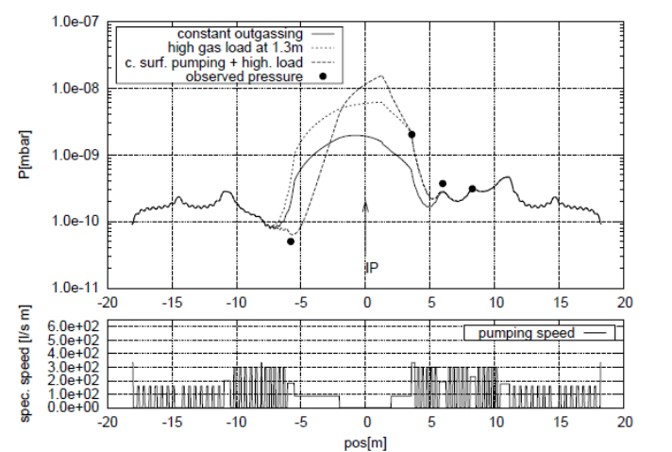
\includegraphics[width=.75	\textwidth]{../../img/hera_badvac_regions.jpg}
	\caption{HERA-II Vacuum pressure distribution around the IP following HERA-II upgrade.  Minima correspond to placement of the vacuum pumps.}
	\label{fig:hera1}
\end{figure}


\begin{figure}
	\centering
	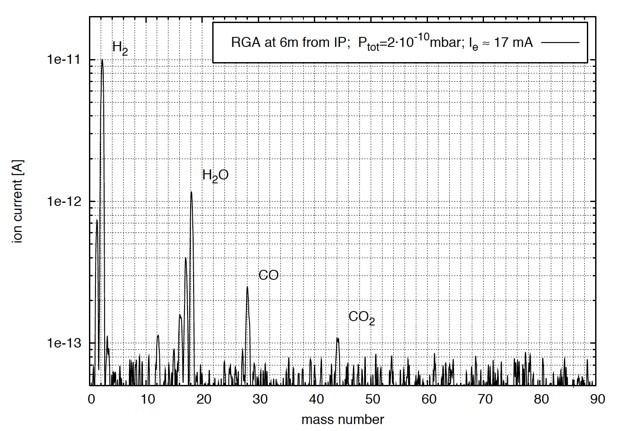
\includegraphics[width=.75\textwidth]{../../img/hera_badvac_comp.jpg}	
	\caption {HERA-II Composition of beampipe gas 6 m from IP. }
	\label{fig:hera2}
\end{figure}

\begin{figure}
	\centering
	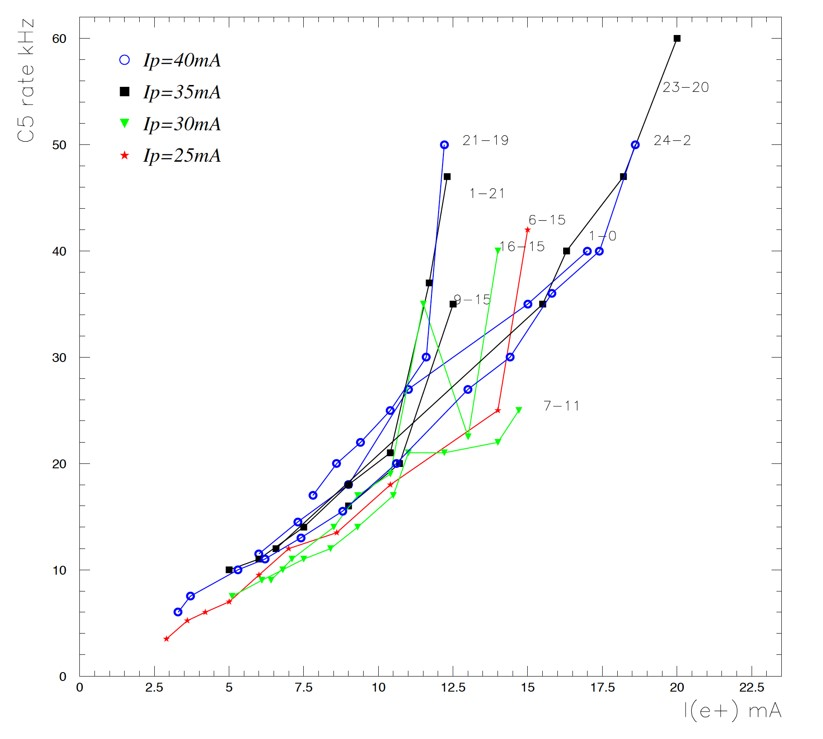
\includegraphics[width=.75\textwidth]{../../img/hera_c5_rate.jpg}
	\caption{C5 rate as a function of HERA \textit{e} beam current for different \textit{p} beam current.  Numeric tags indicate the date and hour of the beginning of \textit{ep} injection for July 2002.}
	\label{fig:hera3}
\end{figure}

\begin{figure}
	\centering
	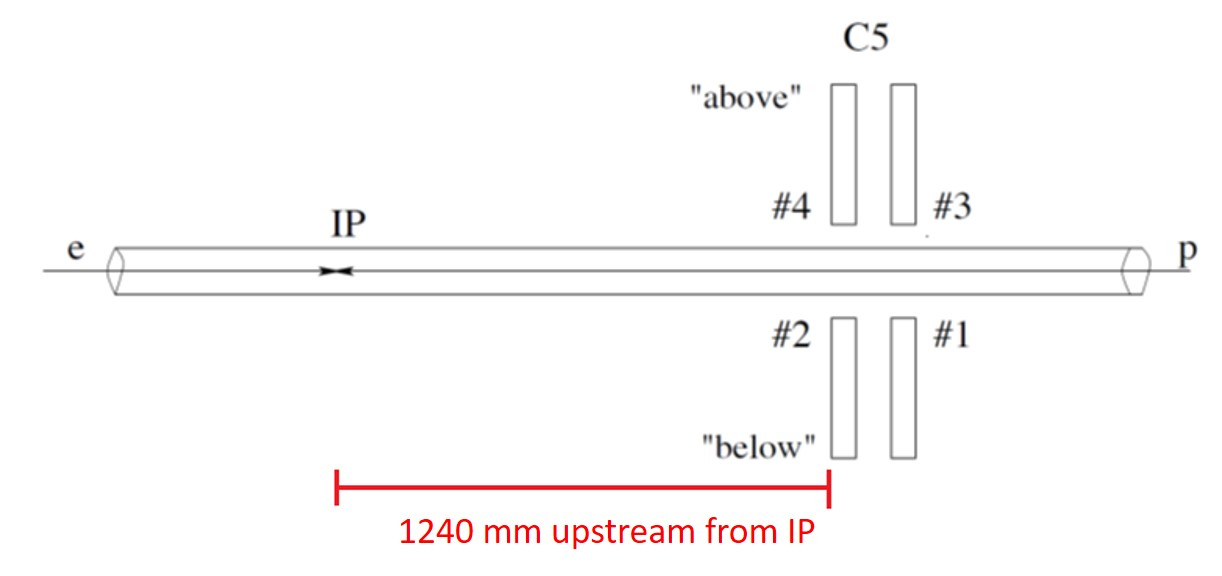
\includegraphics[width=.75\textwidth]{../../img/c5_placement.jpg}
	\caption{C5 detector placement along HERA beamline.}
	\label{fig:hera4}
\end{figure}


\begin{figure}
	\centering
	\begin{minipage}{0.45\textwidth}
		\centering
		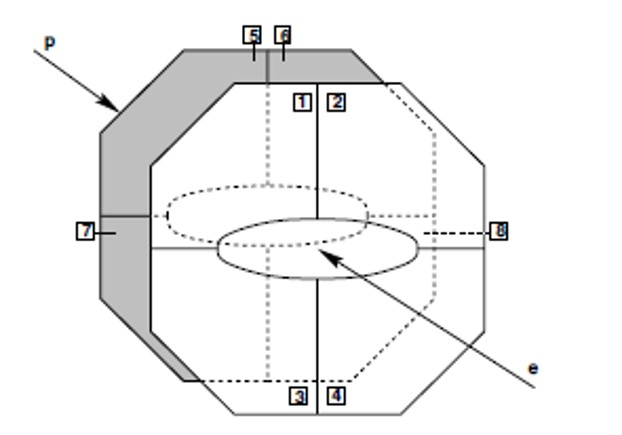
\includegraphics[width=.75\textwidth]{../../img/hera_c5.jpg}
		\caption {Left: Schematic of the actual C5 Time of Flight Detector  }
		\label{fig:hera5}
	\end{minipage}\hfill
	\begin{minipage}{0.45\textwidth}
		\centering	\includegraphics[width=.75\textwidth]{../../img/C5_gemc}	
		\caption {Virtual C5 detector rendered in GEMC.}
		\label{fig:hera6}
	\end{minipage}
\end{figure}




%\begin{figure}
%	\centering
%	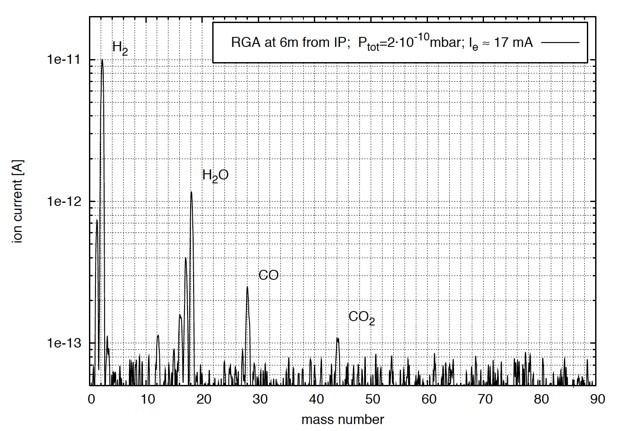
\includegraphics[width=.75\textwidth]{../../img/hera_badvac_comp.jpg}
%	\caption{HERA-II Vacuum pressure distribution in the IR.  The vacuum in the region $\pm$ 5m around the IP deteriorated to $10^{-8}$ mbar, compared to $10^{-10}$ mbar achieved at the pump locations.}
%	\label{fig:hera1}
%\end{figure}

%\begin{figure}
%	\centering
%	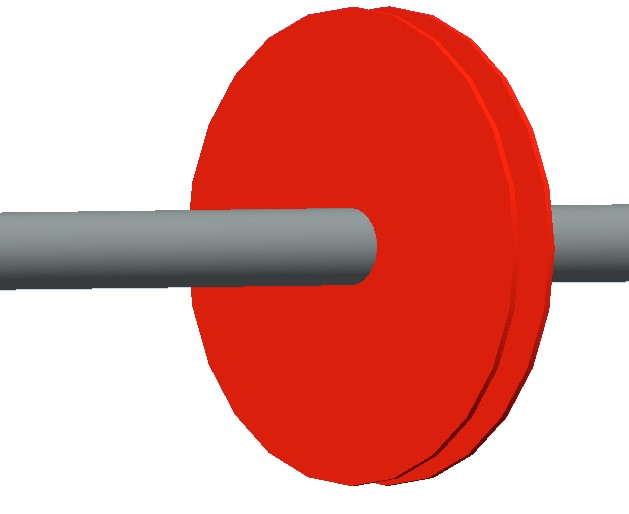
\includegraphics[width=.75\textwidth]{../../img/c5_gemc.jpg}
%	\caption{HERA-II Vacuum pressure distribution in the IR.  The vacuum in the region $\pm$ 5m around the IP deteriorated to $10^{-8}$ mbar, compared to $10^{-10}$ mbar achieved at the pump locations.}
%	\label{fig:hera1}
%\end{figure}

%\begin{figure}
%	\centering
%	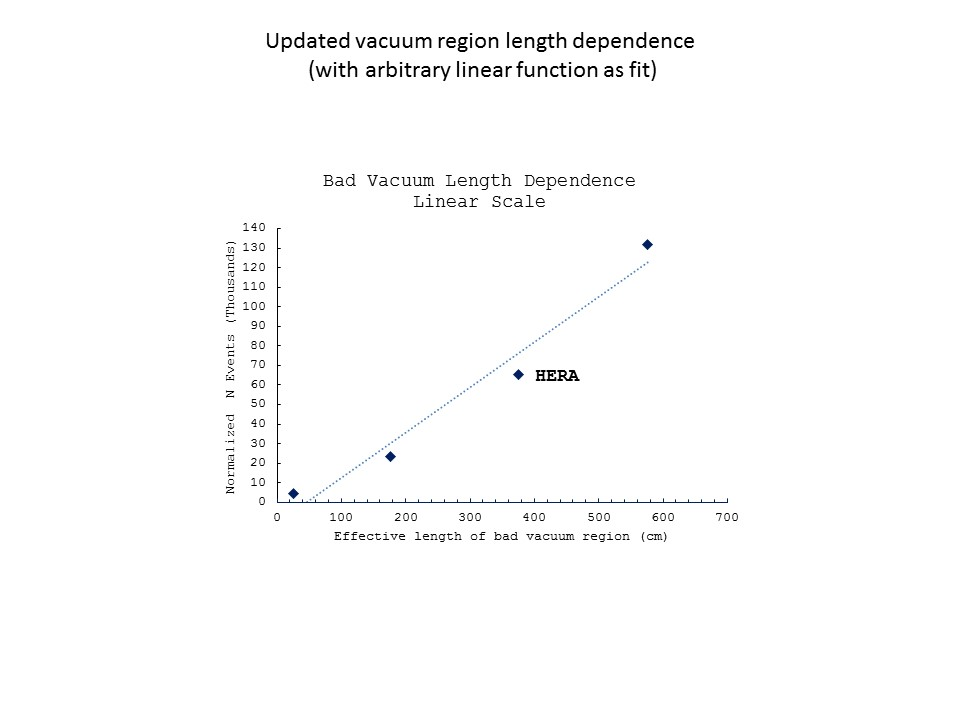
\includegraphics[width=.75\textwidth]{../../img/length_dep_linear.JPG}
%	\caption{HERA-II Vacuum pressure distribution in the IR.  The vacuum in the region $\pm$ 5m around the IP deteriorated to $10^{-8}$ mbar, compared to $10^{-10}$ mbar achieved at the pump locations.}
%	\label{fig:hera1}
%\end{figure}

%\begin{figure}
%	\centering
%	\includegraphics[width=.75\textwidth]{../../img/ length_dep_log.JPG}
%	\caption{HERA-II Vacuum pressure distribution in the IR.  The vacuum in the region $\pm$ 5m around the IP deteriorated to $10^{-8}$ mbar, compared to $10^{-10}$ mbar achieved at the pump locations.}
%	\label{fig:hera1}
%\end{figure}

%\begin{figure}
%	\centering
%	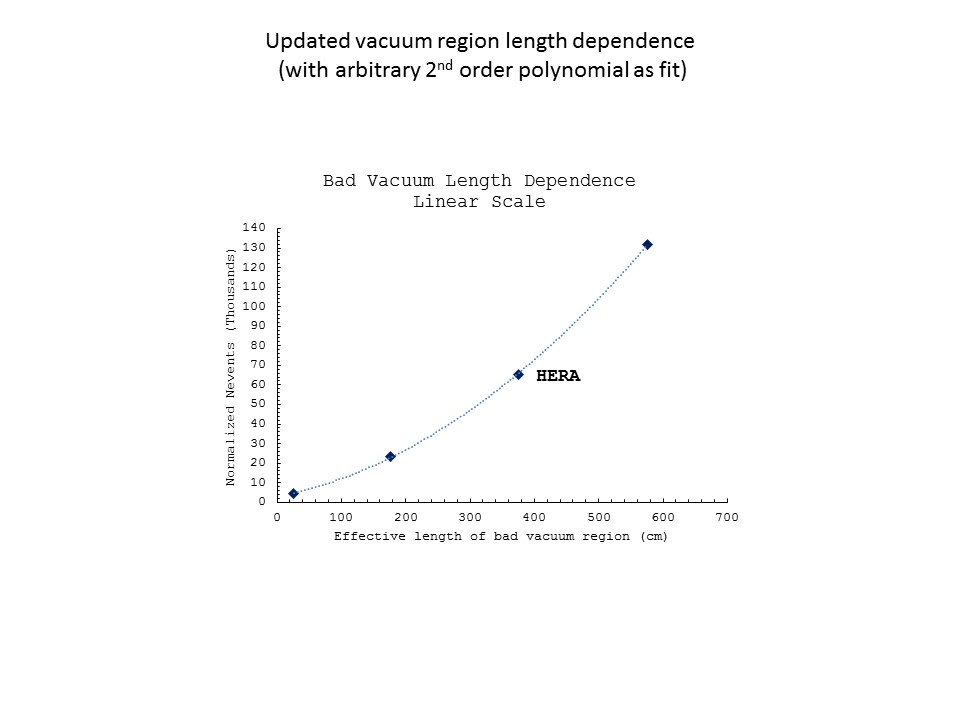
\includegraphics[width=.75\textwidth]{../../img/length_dep_poly.JPG}
%	\caption{HERA-II Vacuum pressure distribution in the IR.  The vacuum in the region $\pm$ 5m around the IP deteriorated to $10^{-8}$ mbar, compared to $10^{-10}$ mbar achieved at the pump locations.}
%	\label{fig:hera1}
%\end{figure}

%\begin{figure}
%	\centering
%	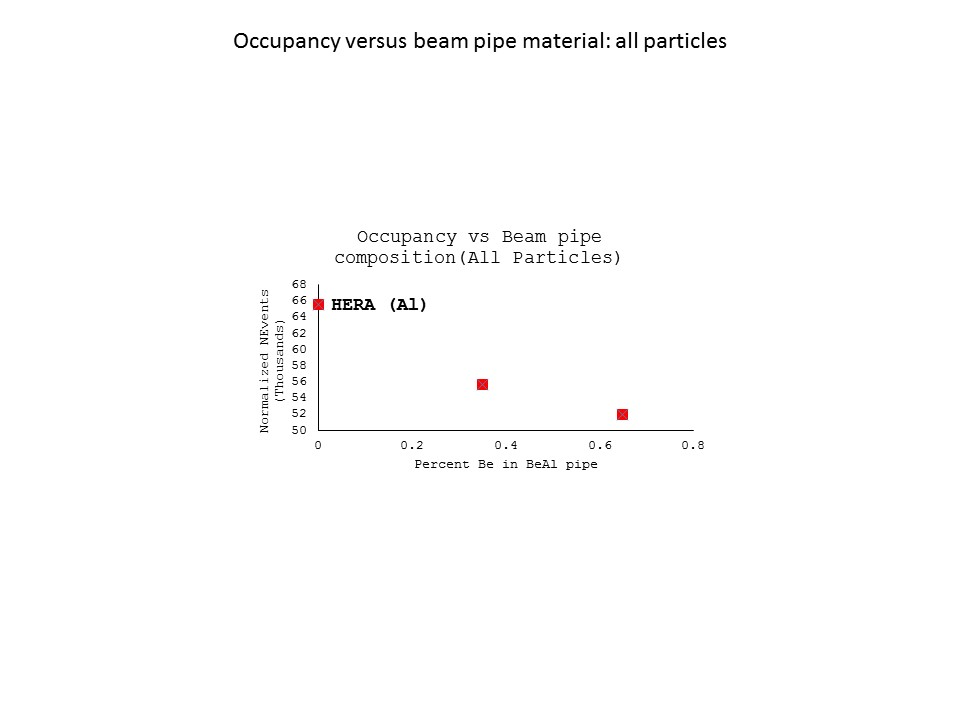
\includegraphics[width=.75\textwidth]{../../img/pipe_comp_all.JPG}
%	\caption{HERA-II Vacuum pressure distribution in the IR.  The vacuum in the region $\pm$ 5m around the IP deteriorated to $10^{-8}$ mbar, compared to $10^{-10}$ mbar achieved at the pump locations.}
%	\label{fig:hera1}
%\end{figure}

%\begin{figure}
%	\centering
%	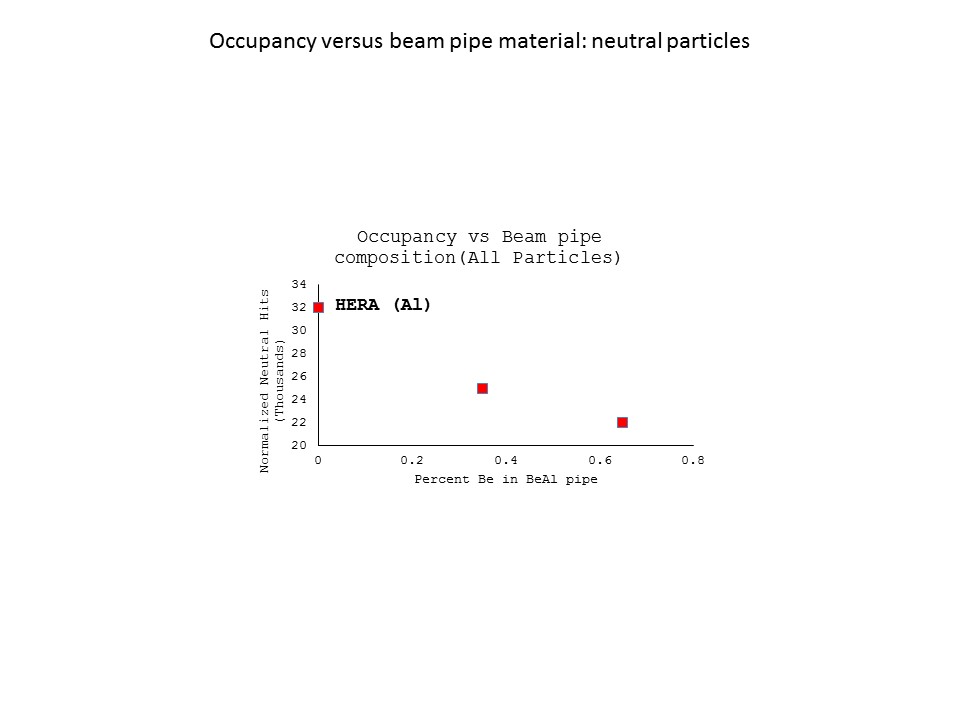
\includegraphics[width=.75\textwidth]{../../img/pipe_comp_neutral.JPG}
%	\caption{HERA-II Vacuum pressure distribution in the IR.  The vacuum in the region $\pm$ 5m around the IP deteriorated to $10^{-8}$ mbar, compared to $10^{-10}$ mbar achieved at the pump locations.}
%	\label{fig:hera1}
%\end{figure}

%Simple table
%\begin{center}
%	\begin{tabular}{ |c|c|c| } 
%		\hline
%		cell1 & cell2 & cell3 \\ 
%		cell4 & cell5 & cell6 \\ 
%		cell7 & cell8 & cell9 \\ 
%		\hline
%	\end{tabular}
%\end{center}